\documentclass[a4paper, 12pt]{report}


\usepackage[czech]{babel} % czech language
\usepackage{pdfpages} % for including pdf files
\usepackage{microtype} % better text rendering
\usepackage[T1]{fontenc} % better text rendering
\usepackage{graphicx} % for images
\usepackage[hidelinks]{hyperref} % for clickable links, hidelinks hides the ugly boxes
\usepackage[a4paper,width=150mm,top=25mm,bottom=25mm,bindingoffset=6mm]{geometry} % page layout
\usepackage[pagestyles]{titlesec} % for customizing chapter titles

% for customizing bibliography title
\addto{\captionsczech}{\renewcommand{\bibname}{Seznam zdrojů}}

% for customizing chapter titles
\titleformat{\chapter}[display]{\normalfont\sffamily\bfseries}{}{0pt}{\Huge}
\newpagestyle{mystyle}
{\sethead[\thepage][][\chaptertitle]{}{}{\thepage}}
\pagestyle{mystyle}

\author{Petr Kotlan}
\title{Optimalizace investičních prostředků z hlediska
výnosu fotovoltaických elektráren}
\date{}

\begin{document}

\begin{titlepage}
    \begin{center}
        \Huge

        % \textbf{Univerzita Jana Evangelisty Purkyně \\v Ústí nad Labem}
        \textbf{\textsf{\textls*[-20]{Univerzita Jana Evangelisty Purkyně \\v Ústí nad Labem}}}
            
        \vspace{1cm}
        \LARGE
        \textbf{\textsf{Přírodovědecká fakulta}}
        
        \vspace{2cm}
        \includegraphics[width=0.5\textwidth]{static/PřF-UJEP-logo.png}
        \vspace{3cm}
            
        \textbf{\textsf{Optimalizace investičních prostředků \\z hlediska výnosu fotovoltaických elektráren}}
        
        \vspace{1cm}

        \large
        BAKALÁŘSKÁ PRÁCE

        \vfill

            \begin{flushleft}
                
            \large
            \textbf{Vypracoval:} Petr Kotlan \\
            \vspace{0.3cm}
            \textbf{Vedoucí práce:} Ing. Roman Vaibar, Ph.D., MBA \\
            \vspace{1.5cm}
            \textbf{Studijní program:} Matematika ve firmách a veřejné správě
        \end{flushleft}

        \vspace{1.5cm}
        
        \LARGE
        Ústí nad Labem 2024

    \end{center}
\end{titlepage}

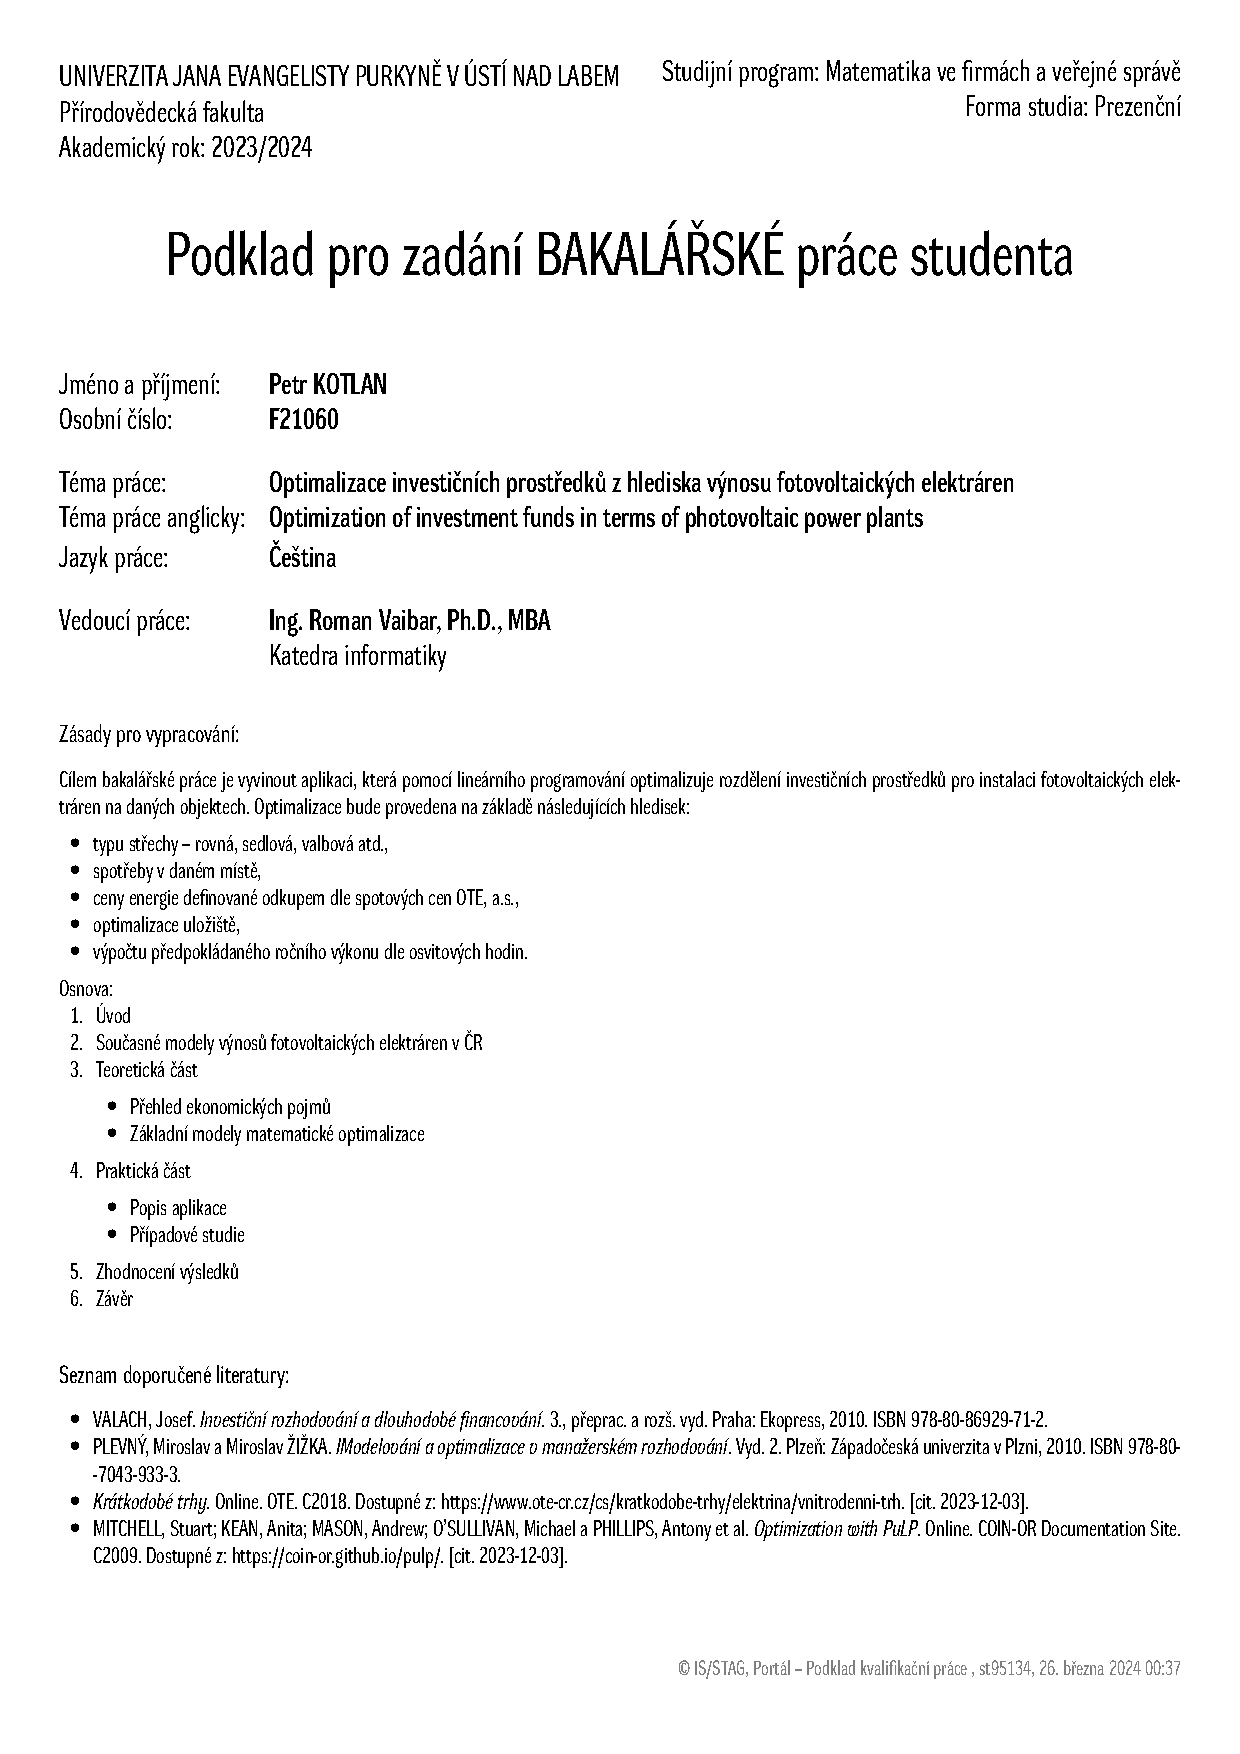
\includepdf[pages=-]{static/podklad_bp.pdf}

\tableofcontents

\addcontentsline{toc}{chapter}{Úvod}
\chapter*{Úvod}

\chapter{Současné modely výnosů fotovoltaických elektráren v ČR}

\chapter{Teoretická část}

\section{Přehled ekonomických pojmů}
Tato část se nejprve zabývá pojmy a ukazateli z oblasti investic.
Poté jsou popsány metody a základní modely lineárního programování.

\section{Investice}

% TODO: citace

Investicí se označuje takové vynaložení finančních prostředků, které se v budoucnu nějakou mírou zhodnotí.
Investice se dělí na reálné a finanční. Mezi reálné patří například investice do nemovitostí, drahých kovů nebo uměleckých děl, tedy do hmotného majetku.
Finanční investice jsou investice do finančních aktiv, jako jsou akcie nebo dluhopisy.
Jako základní pomůcka k posouzení investic slouží \textit{investiční trojúhelník}, který zahrnuje tři základní parametry investice: rizikovost, výnosnost a likviditu.
Obecně platí, že s rostoucím výnosem roste rizikovost a klesá likvidita a naopak.

\subsection{Investiční možnosti}

Záměrem je porovnat investici do fotovoltaické elektrárny s jinými možnostmi.
% vysvetlit proc bereme pouze financi investice


\subsubsection{Spořící účty}
mají zpravidla vyšší úrokovou sazbu než běžné účty.
Výhodou je vysoká likvidita.
V současnosti se úroková sazba pohybuje okolo 4.5\% p.a.

\subsubsection{Dluhopisy} jsou cenné papíry,
které držiteli garantuje pravidelný výnos a jeho následný zpětný odkup.
Známým druhem dluhopisů jsou státní dluhopisy, které Ministerstvo financí prodává několika největším bankám a obchodníkům.
Ti je pak prodávají dalším zájemcům.


\subsubsection{Akcie} je cenný papír, který představuje podíl na kapitálu akciové společnosti.
Majitel akcií má právo na tzv. \textit{dividenda}, tedy podíl na zisku společnosti.


\subsection{Ukazatele výnosnosti investice}

Ukazatele výnosnosti investic jsou klíčovými nástroji při hodnocení investičních rozhodnutí
Poskytují investorům přehled o efektivitě investice a umožňují vzájemné porovnání různých investičních příležitostí.



\subsubsection{Výnosnost investice}
($ROI$ -- Return of Investment)
% https://www.moneta.cz/slovnik-pojmu/detail/roi
vyjadřuje zisk nebo ztrátu z investice v procentech.

\begin{equation}
    ROI = \frac{(P_1 + P_2 + \ldots + P_t) - K}{K} \cdot 100,
\end{equation}

kde
\begin{itemize}[label={}]
    \item $t$ -- počet let,
    \item $P_1, P_2, \ldots, P_t$ -- peněžní příjmy z investice v jednotlivých letech,
    \item $K$ -- kapitálový výdaj,
    \item $ROI$ -- návratnost investice.
\end{itemize}

\subsubsection{Diskontované cash-flow}
($DCF$ -- Discounted Cash Flow)
vyjadřuje současnou hodnotu budoucích peněžních toků.

\begin{equation}
    DCF = \frac{P_1}{(1+i)} + \frac{P_2}{(1+i)^2} + \ldots + \frac{P_t}{(1+i)^t},
\end{equation}

kde
\begin{itemize}[label={}]
    \item $t$ -- počet let,
    \item $P_1, P_2, \ldots, P_t$ -- peněžní příjmy z investice v jednotlivých letech,
    \item $i$ -- úroková míra (diskontní sazba),
    \item $DCF$ -- diskontované cash-flow.
\end{itemize}

\subsubsection*{Čistá současná hodnota}
($NPV$ -- Net Present Value)
vyjadřuje současnou hodnotu budoucích peněžních toků po odečtení kapitálového výdaje.

\begin{equation}    
NPV = \frac{P_1}{(1+i)} + \frac{P_2}{(1+i)^2} + \ldots + \frac{P_t}{(1+i)^t} - K,
\end{equation}

kde
\begin{itemize}[label={}]
    \item $t$ -- počet let,
    \item $P_1, P_2, \ldots, P_t$ -- peněžní příjmy z investice v jednotlivých letech,
    \item $K$ -- kapitálový výdaj,
    \item $i$ -- úroková míra (diskontní sazba),
    \item $NPV$ -- čistá současná hodnota.
\end{itemize}

\subsubsection*{Vnitřní výnosové procento}
($IRR$ -- Internal Rate of Return)
je úroková míra, při níž se současná hodnota peněžních příjmů z investice rovná kapitálovým výdajům. Investice se považuje za výhodnou, když $IRR$ představuje vyšší úrok, než je požadovaná minimální výnosnost investice.

\begin{equation}
    \frac{P_1}{(1+IRR)} + \frac{P_2}{(1+IRR)^2} + \ldots + \frac{P_t}{(1+IRR)^t} = K,
\end{equation}

kde
\begin{itemize}[label={}]
    \item $t$ -- počet let,
    \item $P_1, P_2, \ldots, P_t$ -- peněžní příjmy z investice v jednotlivých letech,
    \item $K$ -- kapitálový výdaj,
    \item $IRR$ -- vnitřní výnosové procento.
\end{itemize}


\section{Základní modely matematické optimalizace}

\chapter{Praktická část}

\section{Popis aplikace}
\subsection{Data}

\subsubsection*{Český hydrometeorologický ústav}

\textbf{ČHMÚ}

\href{https://www.chmi.cz/files/portal/docs/meteo/ok/open_data_2023/Podminky_uziti_udaju.pdf}{Podmínky užití dat}

\subsubsection*{OTE, a.s.}

OTE (Otevřený trh s elektřinou)



\section{Případové studie}

\chapter{Zhodnocení výsledků a závěr}

\addcontentsline{toc}{}{Seznam zdrojů}
\begin{thebibliography}{9}
    \bibitem{demel}
    DEMEL, Jiří. \textit{Operační výzkum}. Dostupné z: \url{https://kix.fsv.cvut.cz/~demel/ped/ov/ov.pdf}.
    
    \bibitem{fotovia-komponenty}
    \textit{Komponenty FVE}. Online. Fotovia. 2023. Dostupné také z: \url{https://www.fotovia.cz/komponenty-fve}.
    
    \bibitem{fotovia-typy}
    \textit{Typy fotovoltaických elektráren}. Online. Fotovia. 2023. Dostupné také z: \url{https://www.fotovia.cz/blog/typy-fotovoltaickych-elektraren}.
    
    \bibitem{ote}
    \textit{Krátkodobé trhy}. Online. OTE. C2018. Dostupné z: \url{https://www.ote-cr.cz/cs/kratkodobe-trhy/elektrina/vnitrodenni-trh}.
    
    \bibitem{tzb-jakfotovoltaikasetripenize}
    \textit{Stroj na peníze: Fotovoltaika při vysokých cenách elektřiny ušetří desetitisíce korun ročně}. Online. TZB-info - Portál pro stavebnictví, technická zařízení budov. 2001. Dostupné z: \url{https://oze.tzb-info.cz/fotovoltaika/24229-stroj-na-penize-fotovoltaika-pri-vysokych-cenach-elektriny-usetri-desetitisice-korun-rocne}.

    \bibitem{tzb-info}
    \textit{Fotovoltaika}. Online. TZB-info - Portál pro stavebnictví, technická zařízení budov. 2001.. Dostupné z: \url{https://oze.tzb-info.cz/fotovoltaika}.

    \bibitem{matematika_pro_ekonomy}
    STOLÍN, Radek. \textit{Matematika pro ekonomy}. 2., upr. vyd. Jihlava: Vysoká škola polytechnická Jihlava, 2011. ISBN ISBN978-80-87035-35-1.

    \bibitem{python-pulp}
    MITCHELL, Stuart; KEAN, Anita; MASON, Andrew; O'SULLIVAN, Michael a PHILLIPS, Antony. \textit{Optimization with PuLP}. Online. COIN-OR Documentation Site. C2009. Dostupné z: \url{https://coin-or.github.io/pulp/}.
    
    \bibitem{moneta}
    \textit{Slovník pojmů z finančnictví a bankovnictví}. Online. MONETA Money Bank. Dostupné z: https://www.moneta.cz/slovnik-pojmu.

    \bibitem{chmu}
    \textit{ČHMÚ}. Online. Dostupné z: \url{https://www.chmi.cz/}.

\end{thebibliography}

\end{document}